% PROGETTAZIONE E CODIFICA

\chapter{Progettazione e codifica}

\section{Progettazione ed implementazione delle \gls{api}}

\subsection{Descrizione dell'architettura}

Dato l'utilizzo dell'architettura \textit{serverless}, non si è applicato nella
scrittura delle \gls{api} alcun tipo particolare di \textit{pattern}.
L'architettura di tipo \textit{serverless} infatti definisce in modo chiaro la
delegazione delle varie responsabilità a componenti molto piccoli e ben
definiti. Questo ha permesso di ottenere tempi di risposta molto brevi.
La parte dedicata alla interazione con gli utenti è stata chiamata
\textit{webhook} a livello progettuale, per distinguerla dalle \gls{api}.

\subsection{Descrizione delle \gls{api}}
Come già accennato nella sezione \ref{prj:serverless:api}, le funzionalità più
importanti sono state suddivise in differenti \gls{api}, ognuna delle quali
risiede in una propria istanza di AWS Lambda.

Comparando questa architettura con un classico pattern
\textbf{MVC}\footnote{\textbf{M}odel \textbf{V}iew \textbf{C}ontroller}, queste
\gls{api} corrisponderebbero al \textit{Model}, che si occupa di gestire parti
della logica della applicazione. Essendo queste parti costituite da una sola
responsabilità e con un solo compito, la loro implementazione si è
concretizzata nella realizzazione di una sola classe per \gls{api}.

\section{Descrizione del \textit{webhook}}
La parte dedicata all'interazione con gli utenti è stata realizzata sempre
usando l'architettura \textit{serverless}, ma essendo la sua complessità
maggiore la strutturazione a classi è stata necessaria al fine di mantenere una
facile comprensione del programma e una buona estendibilità. Tuttavia, per la
natura del servizio che PastBot ricopre, si è scelto di usare una modellazione
ad eventi per gestire le richieste provenienti dalla piattaforma Facebook
Messenger. In base agli eventi che vengono gestiti PastBot si occupa di fare le
chiamate alle \gls{api} corrette. Comparandolo con il pattern di tipo
\textbf{MVC}, \textit{webhook} si occupa di ricoprire la \textit{View} e il
\textit{Controller}.

\section{Descrizione delle classi}
Di seguito si eseguirà una descrizione delle classi più significative che
compongono PastBot e le relative \gls{api}, suddivise in base alla componente
alla quale appartengono.

\begin{figure}[H]
  \centering
  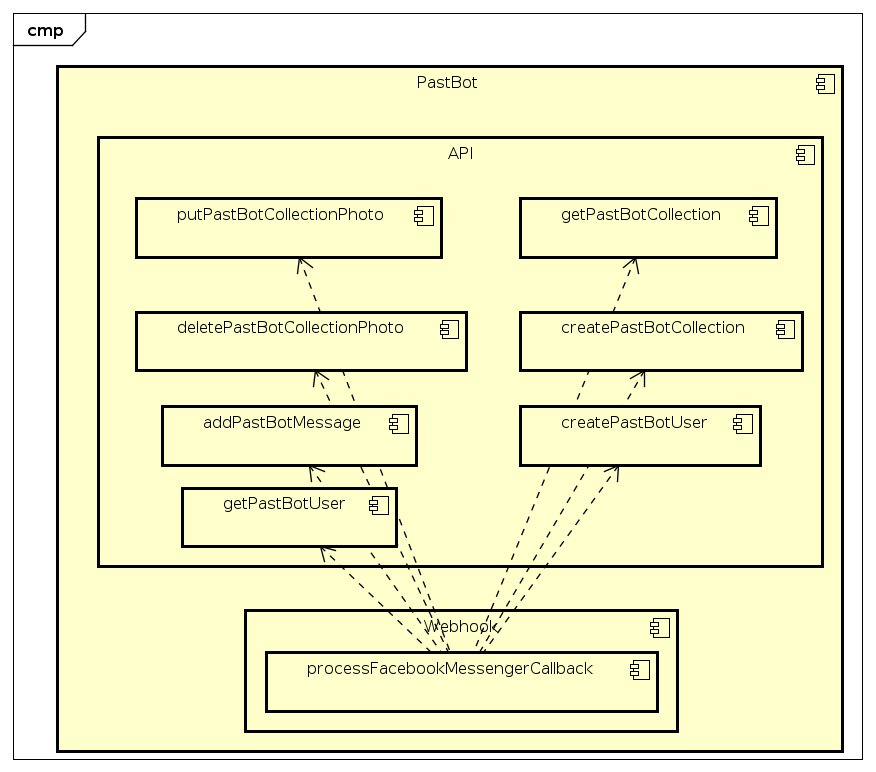
\includegraphics[scale=0.5]{design/overallDesign}
  \caption{Progettazione generale dell'applicazione}
\end{figure}

\subsection{API}
\label{design:api}

Le classi che appartengono a questa componente hanno lo scopo di eseguire le
operazioni sulla base di dati di PastBot. Avendo un solo scopo e una sola
responsabilità, son risultate di facile progettazione.
Per evitare ripetizioni, è riportato qui uno schema generico di una classe
di una \gls{api}:

\begin{figure}[H]
  \centering
  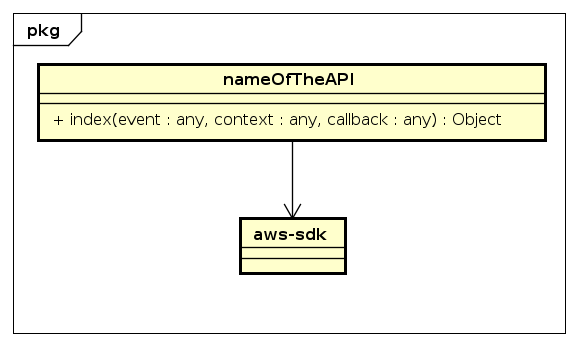
\includegraphics[scale=0.6]{design/singleAPI}
  \caption{Rappresentazione UML di una \gls{api}}
\end{figure}

\label{design:api:params}
È importante segnalare come il servizio Amazon AWS Lambda passi sempre tre
parametri al metodo che andrà a invocare. Questi metodi sono:
\begin{itemize}
  \item \textbf{event}: è un oggetto in formato
\glslink{javascript_object_notation}{JSON} che contiene i campi dell'evento che
viene inviato alla funzione Lambda. Questi campi possono essere definiti in
maniera specifica tramite APIGateway.
  \item \textbf{context}: il programma in esecuzione può usare questo parametro
al fine di poter ottenere informazioni a tempo di esecuzione sul tipo di
funzione Lambda che si sta eseguendo.
  \item \textbf{callback}: tramite questo parametro è possibile, se necessario,
ritornare dati (in formato \glslink{javascript_object_notation}{JSON}) al
chiamante o segnalare uno stato di errore durante l'esecuzione. Essendo questo
parametro opzionale, se non se ne farà uso la risposta che il chiamante otterrà
sarà un valore nullo.
\end{itemize}

\subsection{api::putPastBotCollectionPhoto}

La classe che implementa \textbf{putPastBotCollectionPhoto} si occupa di
aggiungere le foto inviate dall'utente direttamente nel database di PastBot.
Essendo la \textit{privacy} un argomento molto importante quando si trattano i
dati personali degli utenti, si è scelto di salvarle indirettamente tramite il
servizio \textit{Filestack}. Questo servizio di salvataggio dati ha permesso
una facile gestione dei dati riservati, compreso il loro caricamento. Il
salvataggio della foto avviene inviando l'indirizzo \gls{url} dell'allegato
fornito da Facebook Messenger direttamente a \textit{Filestack}.


Questa classe per funzionare necessita del modulo nativo aggiuntivo chiamato
\textit{https}, che permette di connettersi a indirizzi web in maniera sicura
per il trasferimento di dati.

\subsection{api::getPastBotUser}

\textbf{getPastBotUser} si occupa di ritornare al chiamante le informazioni
sull'utente richieste. Viene eseguita quindi una interrogazione del database
degli utenti, in cui verrà cercato l'\textit{id} fornito nell'oggetto della
richiesta. Se l'utente viene trovato, verranno ritornate le informazioni su di
esso e anche la lista degli album (denominati anche \textit{collection}) creati
da quell'utente tramite il \textit{bot}.
Se l'utente non è presente nella base di dati viene ritornato nell'oggetto uno
stato di errore.

\subsection{api::getPastBotCollection}

La responsabilità di \textbf{getPastBotCollection} è di ritornare le
informazioni sull'ultimo album attivo. È necessario fornire l'\textit{id}
dell'utente per poter ottenere l'informazione.
Se viene fornito un \textit{id} non valido o non presente nella base di dati di
PastBot verrà ritornato nell'oggetto di ritorno uno stato di errore.

\subsection{api::createPastBotUser}

Il componente accetta un nuovo utente e si occupa di aggiungerlo alla lista
degli utenti presenti nella base di dati di PastBot. È necessario passare un
identificativo che sia univoco per quell'utente. Se viene passato un
identificativo che è già presente nella base di dati la classe si occuperà di
ritornare al chiamante uno stato di errore.

\subsection{api::deletePastBotCollectionPhoto}

La responsabilità che \textbf{deletePastBotCollectionPhoto} assolve è quella di
cancellare tutte le foto presenti all'interno di un album dato. La
cancellazione sancisce l'eliminazione completa dai database di PastBot e dal
servizio \textit{Filestack}.
Lo stato della cancellazione viene riportato nell'oggetto che verrà ritornato
al chiamante.

\subsection{api::addPastBotMessage}

\textbf{addPastBotMessage} ha l'incarico di salvare il messaggio ricevuto nella
base di dati. Questa funzione serve in futuro a PastBook per poter eseguire
raccolta dati e studi su di essi.

\subsection{api::createPastBotCollection}

L'utilità di questo componente è quella di creare un nuovo album dato un
utente esistente. Se l'identificativo dell'utente non è valido verrà ritornato
un messaggio di errore, altrimenti verrà creato un nuovo album, che porterà a
sua volta un identificativo univoco.

\subsection{\textit{Webhook}}

Le classi all'interno di questo componente si occupano di gestire l'intera
interazione con gli utenti, dalla ricezione del messaggio fino al suo invio. Le
operazioni relative al salvataggio e recupero di informazioni sono effettuate
tramite le \gls{api} illustrate in \ref{design:api}, creando quindi un livello
di indirettezza e una maggiore estendibilità.
Il nome \textit{webhook} è stato dato per differenziare il \textit{bot} dalle
\gls{api}. Essendo infatti il \textit{bot} scritto con le stesse tecnologie
delle \gls{api} si è dovuto porre una differenza a livello di nome, per evitare
incomprensioni.

\begin{figure}[H]
  \centering
  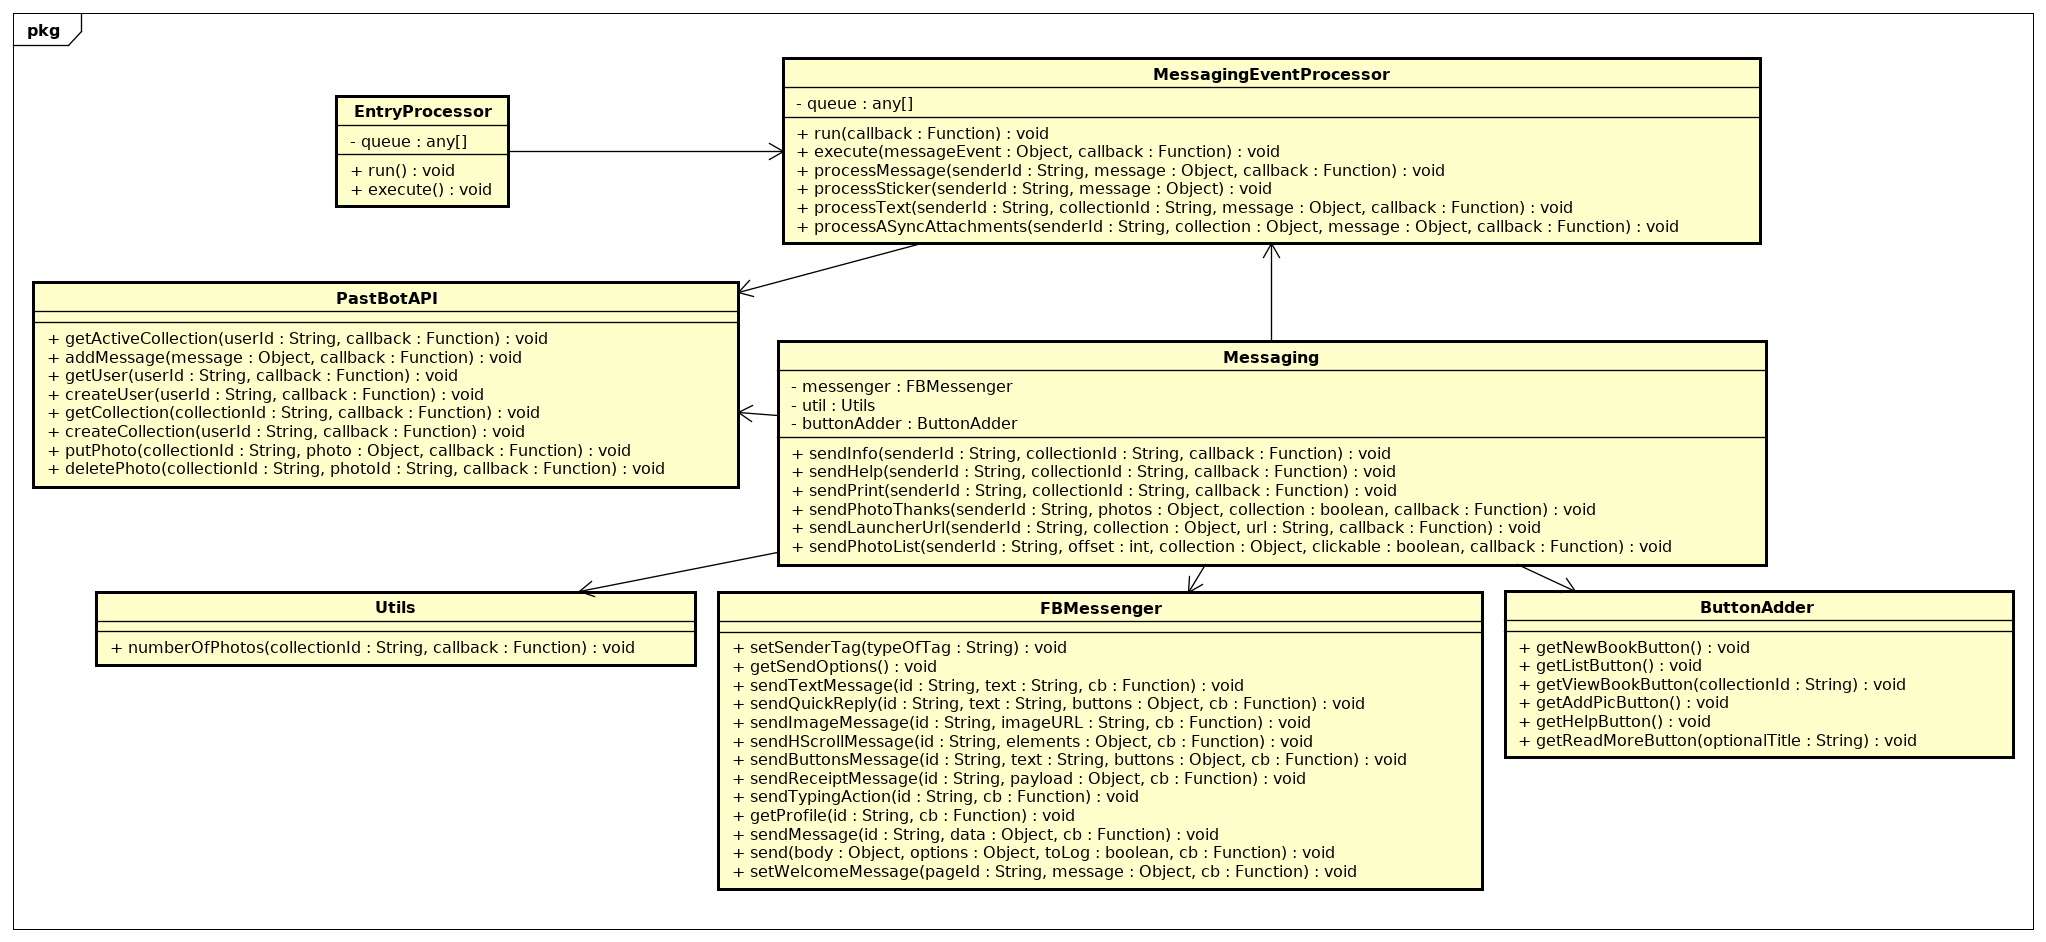
\includegraphics[scale=0.285]{design/processFacebookMessengerCallback}
  \caption{Diagramma delle classi per la parte di PastBot relativa
all'interazione con gli utenti.}
\end{figure}

Messenger attua una politica di concatenazione dei messaggi in arrivo: se un
utente invia per esempio due messaggi in rapida successione, viene generato un
solo evento, che conterrà un \textit{array} di messaggi inviati dall'utente. È
quindi stato creato inizialmente una classe \textbf{EntryProcessor} la quale si
occupa di ricevere l'evento e di estrarne i messaggi che vengono posti in una
coda di esecuzione.
Questa coda viene quindi passata alla classe \textbf{MessagingEventProcessor},
che si occupa di elaborare singolarmente e in maniera asincrona ogni messaggio
presente nella lista. In questa maniera, vengono gestiti diversi eventi nello
stesso tempo di esecuzione, velocizzando il tempo di risposta e diminuendo il
tempo di attesa. Un svantaggio di questa scelta è che le richieste,
essendo processate in maniera indipendente, possono venire ritornate in maniera
non ordinata. Si è comunque scelto di mantenere un approccio asincrono in
quanto è stato ritenuto più importante avere una buona velocità di risposta.

Per ogni messaggio ottenuto si identifica il tipo di messaggio, e in base al
tipo di messaggio viene chiamato il metodo adatto. Grazie al modulo NPM
\textit{Dashbot} è possibile storicizzare i dati ricevuti per poterne poi
eseguire un'analisi dettagliata.
I tipi di messaggi che l'utente può inviare su Messenger sono i seguenti:
\begin{itemize}
  \item messaggio di testo;
  \item \textit{sticker};
  \item allegati.
\end{itemize}
I messaggi di testo vengono ulteriormente analizzati nel metodo
\textbf{processText} che individua specificatamente il tipo di comando che
l'utente ha mandato. Questa sezione è stata studiata in maniera tale che in
futuro possa essere integrato facilmente un sistema per interpretare il
linguaggio naturale, in maniera tale da avere una miglior comprensione delle
richieste effettuate dagli utenti.

Il metodo \textbf{processASyncAttachments} si occupa dell'invio delle foto
alla rispettiva \gls{api}. L'invio delle foto viene effettuato in maniera
asincrona tramite l'utilizzo della classe \textit{Promise} messa a disposizione
dal linguaggio JavaScript. Vengono effettuate multiple chiamate alla stessa
\gls{api} tramite la classe \textbf{PastBotAPI}, che si occupa di prelevare le
immagini inviate dall'utente e inoltrarle alle \gls{api} messe a disposizione
dal servizio di salvataggio file \textit{Filestorage}.
L'allegato non viene direttamente inviato al \textit{bot}: Messenger invia
l'\gls{url} dell'allegato permettendo di velocizzare ulteriormente le
operazioni, in quanto si manipola una stringa e non un file binario che
potrebbe essere più oneroso da processare.

\textbf{processSticker} ha la responsabilità di occuparsi degli \textit{sticker}
ricevuti. Se lo \textit{sticker} inviato è il simbolo del classico "mi piace"
di Facebook PastBot risponderà nella stessa maniera, altrimenti, verrà inviato
un altro simbolo, in maniera tale da mantenere la conversazione attiva e
intrattenere l'utente.

\paragraph*{La classe Messaging} Questa classe si occupa di inviare i messaggi
in risposta all'utente. Per effettuare questa operazione si utilizza la classe
\textbf{FBMessenger}, che permette in questa maniera di fornire un ulteriore
livello di indirettezza. Le classi \textbf{ButtonAdder} e \textbf{Utils} sono
state create per dividere le responsabilità presenti nella classe
\textbf{Messaging}. \textbf{ButtonAdder} si occupa della creazione e
restituzione dei bottoni grafici che poi verranno visualizzati dagli utenti.
Questi bottoni devono essere degli oggetti di tipo
\glslink{javascript_object_notation}{JSON} che seguano quanto specificato dalla
documentazione di Messenger.
\textbf{Utils} contiene un metodo per ottenere il numero di foto presenti in un
album. Questo metodo è stato utilizzato soprattutto per segnalare all'utente il
numero delle foto attualmente caricate e aiutarlo nel raggiungere la soglia
minima per poter acquistare un album.

\paragraph*{La classe FBMessenger} La responsabilità di questa classe è, come
già accennato, quella di inviare i messaggi agli utenti. Il metodo
\textbf{send} si occupa di inviare i dati alle \gls{api} di Messenger. Tutti gli
altri metodi impostano i dati da inviare, contenendo il testo del messaggio
formulato in base alle proprietà che l'utente detiene. Da qui tramite il modulo
NPM per le statistiche \textit{Dashbot} si salvano i messaggi inviati dal
\textit{bot}. A ogni messaggio che il \textit{bot} invia si applica un tipo
particolare di etichetta. In questa maniera nelle statistiche è possibile
conoscere il tipo di messaggio più inviato da parte del \textit{bot}.
